\graphicspath{{figs/App-GaDiss/}}
\chapter{Gaussian Probability Distribution Functions}
\label{app:gaDiss}

\section{Univariate Gaussian Distribution}

A random variable $u$ that assumes values $u_o$ drawn from a Gaussian distribution $G(\mu,\sigma)$ is referred to as a Gaussian random variable and is denoted as $u \sim G(\mu,\sigma)$.
The univariate Gaussian distribution $G(\mu,\sigma)$, also referred to as the normal distribution, is defined as:
\begin{equation}
	G(u\,;\,\mu,\sigma) \triangleq \frac{1}{\sqrt{2\pi\sigma^2}} \exp\left[-\frac{1}{2\sigma^2}(u-\mu)^2\right]
	\label{eqn:gassDisUnivar}
\end{equation}
where $\mu$ and $\sigma^2$ are referred  as the mean and the variance of the Gaussian distribution correspondingly, while $\sigma$ is referred to as the standard deviation.
The term $1/\sqrt{2\pi\sigma^2}$ is the normalization constant that ensures the property $\int_{-\infty}^{\infty} G(u\,;\,\mu,\sigma)\, \mathrm{d}u = 1$.
As a result, the Gaussian distributions, in their basic form, are fully characterized by their mean and variance parameters.
\figRef{fig:gauPlot} illustrates different Gaussian distribution plots for different $\mu$ and $\sigma$ parameters.
Notice that the Gaussian distribution has a maximum value at its mean point $u=\mu$.
\begin{figure}
	\centering{
	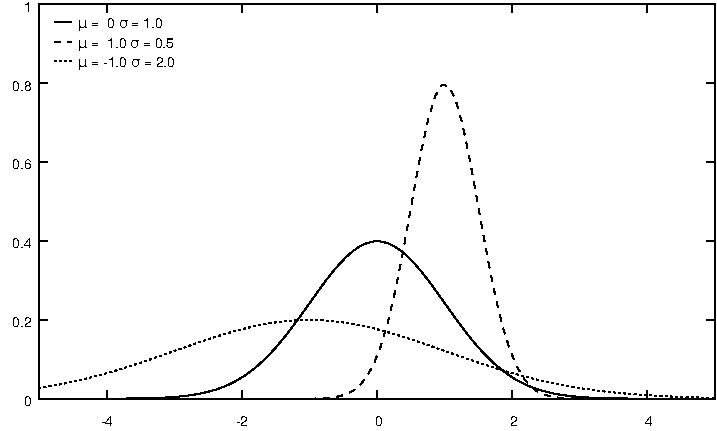
\includegraphics[scale=1.0]{gauPlot}
	}
	\caption[Sample univariate Gaussian distribution plots.]{Sample univariate Gaussian distribution plots for different $\mu$ and $\sigma$ values.}
	\label{fig:gauPlot}
\end{figure}


The Gaussian distribution used in the derivation of the \gls{acr:fgabp} algorithm in \secRef{chp:FGaBP} can more conveniently be represented using a parameterization referred to as the canonical parameterization, or the information form.
The Gaussian distribution can also be used in an un-normalized form by ignoring the normalizing constant.
This does not constitute any loss of information since the Gaussian distribution is fully identified by its mean and variance parameters or, correspondingly, the canonical $\beta$ and $\alpha$ parameters.
The un-normalized canonical representation of the univariate Gaussian distribution is defined as:
\begin{equation}
	G(u\,;\,\beta,\alpha) \propto \exp\left[-\frac{1}{2}\alpha u^2 + \beta u\right]
	\label{eqn:gassDisUnivarCan}
\end{equation}
where $\alpha = 1/\sigma^2$ is the reciprocal of the variance, also referred to as the precision; and $\beta = \mu/\sigma^2$ is the second canonical parameter.


\section{Multivariate Gaussian Distribution}

A collection of $n$ random variables $U=(u_1,u_2,\cdots,u_n)$ have a joint Gaussian probability distribution ($U\sim\mathcal{G}(\bar{\mu},\Sigma)$)  defined as:
\begin{equation}
	\mathcal{G}(U\,;\,\bar{\mu},\Sigma) \triangleq \frac{1}{(2\pi)^{n/2}|\Sigma|^{1/2}} \exp\left[-\frac{1}{2}(U-\bar{\mu})^T\Sigma^{-1}(U-\bar{\mu})\right]
	\label{eqn:gausDisMult}
\end{equation}
where $\bar{\mu}$ is the mean vector of size $n$ for the joint Gaussian random variables $U$; $\Sigma$ is the covariance matrix; and $|\cdot|$ is the determinant operator.
The covariance matrix $\Sigma$ must be \acrfull{acr:spd} in order for $\mathcal{G}$ to be a valid Gaussian probability distribution.
\figRef{fig:gauPlot3D} illustrates a sample bivariate Gaussian distribution plot with $\bar{\mu} = (0.5,0.5)$ and $\Sigma=I$, where $I$ is the identity matrix.
A key property of Gaussian distributions is that they hold their maximum value at $U=\bar{\mu}$.
\begin{figure}
	\centering{
	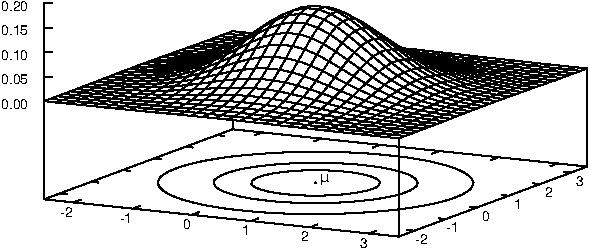
\includegraphics[scale=1.0]{gauPlot3D}
	}
	\caption[Sample bivariate Gaussian distribution plot.]{Sample bivariate Gaussian distribution plot with $\bar{\mu} = (0.5,0.5)$ and $\Sigma=I$.}
	\label{fig:gauPlot3D}
\end{figure}


Similar to the univariate case, the multivariate Gaussian distribution can be represented in the un-normalized canonical form as:
\begin{equation}
	\mathcal{G}(U\,;\,\bar{\mu},\Sigma) \propto \exp\left[-\frac{1}{2}U^T W U + K^T U \right]
	\label{eqn:gausDisMultCan}
\end{equation} 
where $W=\Sigma^{-1}$ is the inverse covariance matrix, also referred to as the precision matrix; and $K=\Sigma^{-1}\bar{\mu}$ is the scaled mean parameter.


The original form of the Gaussian distribution in \eqnRef{eqn:gassDisUnivar} and \eqnRef{eqn:gausDisMult} can be obtained from \eqnRef{eqn:gassDisUnivarCan} and \eqnRef{eqn:gausDisMultCan} correspondingly by completing the algebraic square of the exponent and adjusting the normalizing constant accordingly.
The canonical form is used in the \gls{acr:fgabp} algorithm in order to produce more convenient formulation when multiplying and marginalizing Gaussian distributions as will be illustrated below.


\section{Multiplication of Gaussian Distributions}

Multiplication of any number of Gaussian distributions results in a Gaussian distribution up to a constant.
Using un-normalized canonical forms, the resulting distribution has canonical parameters equal to the sum of the canonical parameters of the multiplied distributions.
The multiplication of $M$ multivariate Gaussian distributions that represent the same Gaussian random variable vector $U$ can be formulated as:
\begin{equation}
	\mathcal{G}(U\,;\,W,K) \propto \prod_{m=1}^{M} \mathcal{G}_m(U\,;\,W_m,K_m)
	\label{eqn:gausDisMultp}
\end{equation}
the resulting distribution $\mathcal{G}$ is Gaussian with canonical parameters computed by:
\begin{align}
	W &= \sum_{m=1}^{M} W_m \\
	K &= \sum_{m=1}^{M} K_m.
\end{align}
This result can readily be applied to scalar Gaussian distributions by replacing the multidimensional parameters with their scalar counterparts.


\section{Marginalization of Gaussian Distributions}

Marginalization of a multivariate Gaussian distribution is integrating away a subset of variables, sometimes referred to as nuisance variables, so that the resulting distribution is a function of the variables of interest.
An important property of Gaussian distributions is that any marginalization of a Gaussian distribution results in a Gaussian distribution.
To further illustrate, suppose that the Gaussian variable vector $U$ is partitioned into two subsets labeled $a$ and $b$ such that $U = (U_a,U_b)$.
Then, to marginalize the Gaussian distribution for $U_a$, we formulate the following:
\begin{equation}
	\mathcal{G}(U_a\,;\,\bar{W_a},\bar{K_a}) \propto \int_{U_b} \mathcal{G}(U\,;\,W,K)\, \mathrm{d}U_b.
	\label{eqn:gausDisMarj}
\end{equation}
To evaluate this integral, we first partition $W$ and $K$ according to the $U_a$ and $U_b$ partitions as follows:
\begin{equation}
	\begin{array}{cc}
		W=\left[%
		\begin{array}{llll}
			W_{aa} & W_{ab} \\
			W_{ba} & W_{bb}
		\end{array}%
		\right],&%
		K=\left[%
		\begin{array}{l}
			K_a \\
			K_b
		\end{array}
		\right].
	\end{array}
	\label{eqn:WKPartitions}
\end{equation}
We then manipulate \eqnRef{eqn:gausDisMarj} by separating the $U_a$ and $U_b$ variables, completing the algebraic square, and using the Gaussian integral identity stated as follows:
\begin{equation}
	\int_U \exp\left[-\frac{1}{2}(U-\mu)^T\Sigma^{-1}(U-\mu)\right]\,\mathrm{d}U = (2\pi)^{n/2}|\Sigma|^{1/2}.
	\label{eqn:GausInteg}
\end{equation}
Finally the integral \eqnRef{eqn:gausDisMarj} is evaluated by finding the $\bar{W_a}$ and $\bar{K_a}$ parameters as follows:
\begin{align}
	\bar{W_a} &= W_{aa} - W_{ab} W_{bb}^{-1} W_{ba}\\
	\bar{K_a} &= K_{a} - W_{ab} W_{bb}^{-1} K_{b}.
	\label{eqn:gausDisMarjWK}
\end{align}
